\section{Analysis}
\label{sec:analysis}
\subsection{Regression analysis}

Using the data in Table \ref{Bt2} and equations \eqref{Be6},\eqref{Be7} to calculate the $Q_o$ and $Q_v$.


\begin{table}[h]
    \centering
    \scalebox{0.9}{
\begin{tabular}{ccccccc}
    \toprule
    $H_{Qv}$ & $H_{Qo}$ &$H_{Qa}$ &$Q_v$  & $Q_o$   & $Q_a$  & $Q_{actual}$  \\
    \midrule
    17&10  &54&0.000102725    & 0.0000953964    & 0.000083333   & 0.0000976 \\
    49&33  &56&0.000174402    &  0.000173296    & 0.000166667    & 0.000173 \\
    107&74  &65&0.000257718    & 0.000259506    &   0.00025    & 0.000251 \\
    195&137  &73&0.000347913    & 0.000353096    & 0.000333333    & 0.000341 \\
    \bottomrule
\end{tabular}}

(Unit of H: $mm$ and Q: $m^3/s$)
\caption{Flow rates measured by different methods}
\label{Bt4}
\end{table}

The regression analysis figure is in figure \ref{Bf4} and data in \ref{Bt5}.

\begin{figure}[h] % Here, top, bottom priority list
    \centering
    \includegraphics[scale=1.1]{Results/B.eps}
    \caption{Regression analysis}
    \label{Bf4}
\end{figure}

\begin{minipage}[h]{\textwidth}
  \begin{minipage}[h]{0.49\textwidth}
    \makeatletter\def\@captype{table}
    \centering
    \scalebox{0.9}{
    \begin{tabular}{l|ll} 
        \hline
            & Slope ($*10^6$)    & R-square \\ \hline
        $Q_v$ & 1.611 & 1  \\
        $Q_o$ & 1.099 & 1   \\
        $Q_a$ & 1.909 & 0.9855   \\\hline       
    \end{tabular}} 
    \caption{result of regression analysis}
    \label{Bt5} 
  \end{minipage}
  \begin{minipage}{0.49\textwidth}
    \makeatletter\def\@captype{table}
    \centering
    \scalebox{0.85}{
    \begin{tabular}{cccc}
        \toprule
    Flowrate(L/min)     & $Q_v$  & $Q_o$   & $Q_a$\\
        \midrule
5 & 2.233992 & 5.277012 & 14.59668 \\
10 & 0.396002 & 1.036594 & 3.444661 \\
15 & 3.22237  & 2.51114  & 0.558865 \\
20 & 3.514961 & 1.99558  & 2.2786 \\
\bottomrule
    \end{tabular}}
    \caption{Error percentage}
    \label{Bt6}
  \end{minipage}  
\end{minipage}


\subsection{Error analysis}
\begin{equation}
    Error=\frac{|Q_v-Q_t|}{Q_t}*100\%
    \label{Be9}
\end{equation}
The results is shown in the table \ref{Bt6}.
The error for each flowmeter is calculated 
by using the final outflow flow rate ($Q_{actual}$) as the criterion.

Here are some of the reasons for the errors

$\bullet$  